\begin{figure*}[ht]
    \centering
    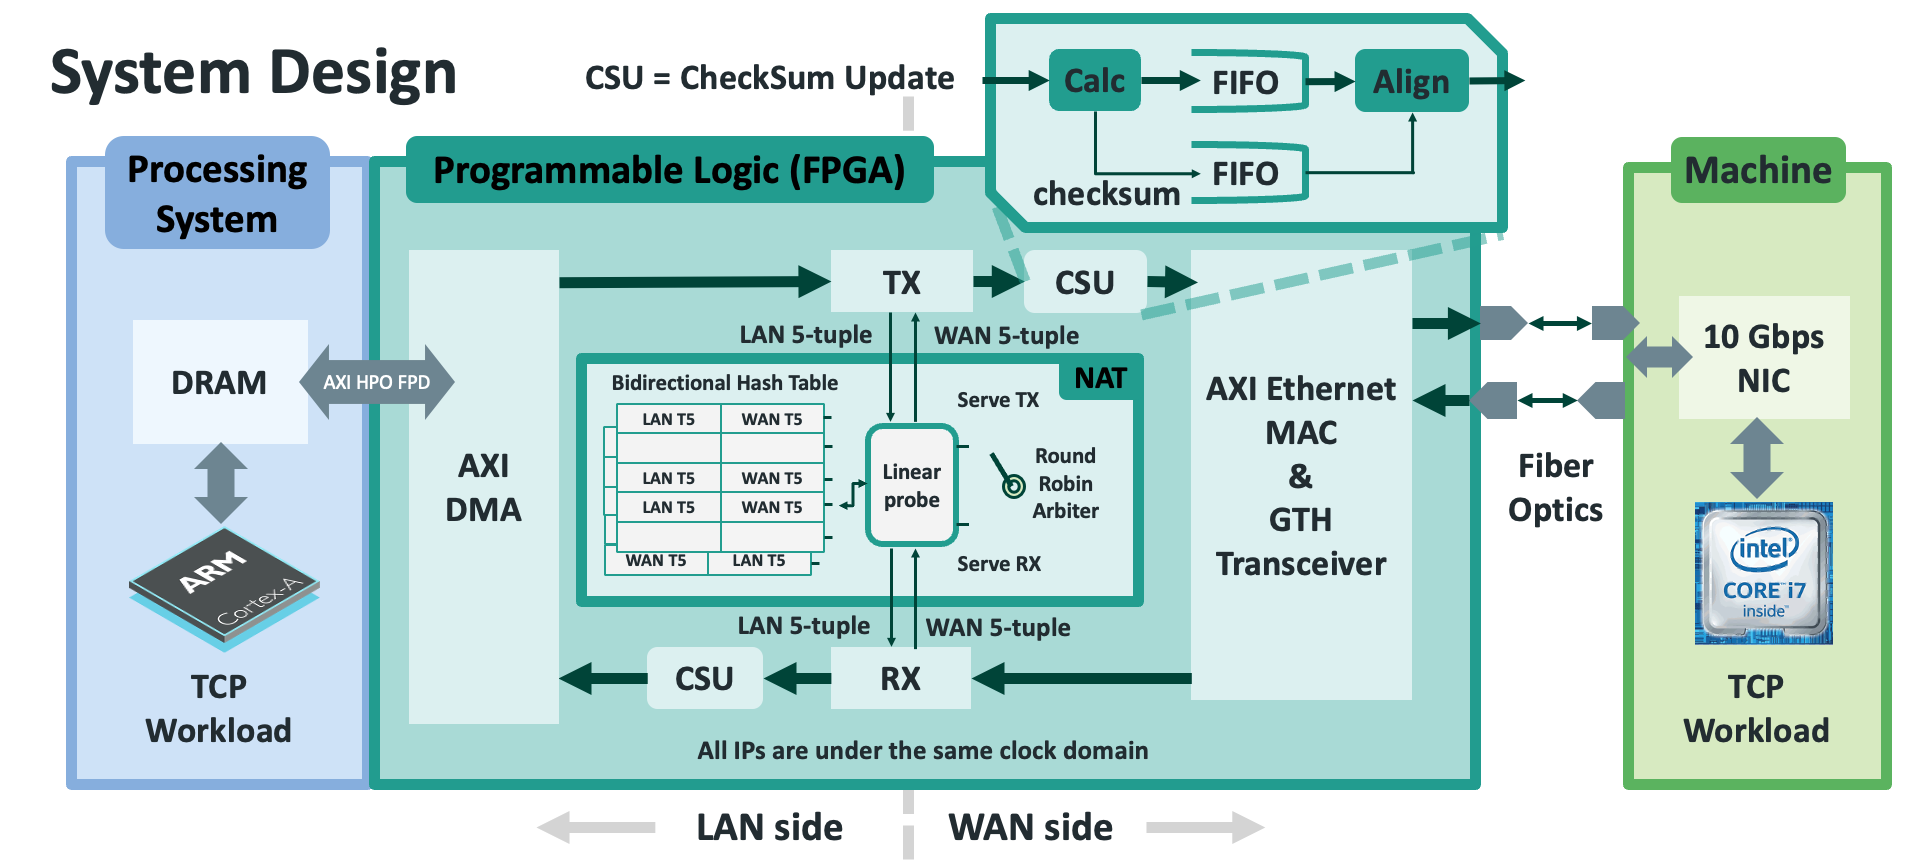
\includegraphics[width=\linewidth]{images/design.png}
    \caption{System Design}
    \label{fig:design}
    \Description{}
\end{figure*}

In this section, we present our system design, which is based on the official example of the Ethernet 10/25G system of Xilinx (referred to as the original design hereafter) \footnote{https://github.com/Xilinx-Wiki-Projects/ZCU102-Ethernet/tree/main/2019.2/pl\_eth\_10g}.

\subsection{Original Block Design}
Before delving into our design, it is essential to provide an overview of the organization of the original design for contextual understanding.

\textbf{Components.} The design integrates the Processing System (PS) and Programmable Logic (PL). The PS in ZCU102 includes four ARM Cortex-A53 processors, capable of handling general-purpose computing tasks and providing control for the entire system. The PL is responsible for implementing custom hardware logic, including components such as DMA, MAC, and GTH, which collectively form a 10GbE network interface on the ZCU102 evaluation board. A Xilinx handmade Linux driver is employed to drive this interface on the PS.

We detail the functions of the components implemented in PL as follows:

\begin{itemize}
    \item \textbf{DMA (Direct Memory Access):} Efficiently transfers data between memory and peripherals without involving the processor, enhancing data throughput and offloading data transfer tasks from the processor.
    \item \textbf{MAC (Media Access Control):} Manages the communication protocol for the Ethernet interface, handling frame formatting, addressing, error detection, and other protocol-related tasks.
    \item \textbf{GTH (Gigabit Transceivers):} Facilitates high-speed serial data communication, enabling the transmission and reception of data at gigabit rates.
\end{itemize}

\textbf{Data Flow.} MAC and GTH handle the transmission of data between the FPGA and the external network. Upon receiving incoming data from MAC and GTH, DMA takes control of the data transfer process and moves it into the designated memory location, allowing further processing by the processor or other system components.

\textbf{AXI4-Stream Signals.} Most signals between the modules adopt the AXI4-Stream protocol, with interfaces appearing in pairs - the slave port (starting with \verb|s_|) and the master port (starting with \verb|m_|). The \verb|ready| signal of the slave and the \verb|valid| signal of the master constitute the primary handshake mechanism, indicating a data transfer when both signals are active.

The exact definitions of these AXI4-Stream signals are as follows:

\begin{itemize}
    \item \verb|s_axis_tdata[63:0]|: Data bus received from the master device, conveying data across the interface.
    \item \verb|s_axis_tkeep[7:0]|: Byte qualifier received from the master device, indicating whether corresponding bytes of the data bus are part of the data stream. A low level indicates an invalid byte.
    \item \verb|s_axis_tvalid|: Signal received from the master device, indicating a valid data transfer.
    \item \verb|s_axis_tlast|: Signal received from the master device, marking the last data transfer and indicating the boundary of the data stream.
    \item \verb|s_axis_tready|: Signal sent to the master device, indicating its readiness to accept a data transfer in the current clock cycle.
    \item \verb|m_axis_tdata[63:0]|: Data bus sent to the slave device, providing data across the interface.
    \item \verb|m_axis_tkeep[7:0]|: Byte qualifier sent to the slave device, indicating whether corresponding bytes of \verb|m_axis_tdata| are part of the data stream. A low level indicates an invalid byte.
    \item \verb|m_axis_tvalid|: Signal sent to the slave device, indicating the reception of a valid data transfer.
    \item \verb|m_axis_tlast|: Signal sent to the slave device, marking the last data transfer and indicating the boundary of the data stream.
    \item \verb|m_axis_tready|: Signal received from the slave device, indicating its readiness to send a data transfer in the current clock cycle.
\end{itemize}

\subsection{TX and RX}
Building upon the original block design, we introduce TX and RX to intercept communication between the MAC/GTH and DMA. TX intercepts communication from DMA to MAC/GTH, while RX intercepts communication from MAC/GTH to DMA. Both TX and RX assess whether an incoming packet is a TCP packet.

If the packet is not a TCP packet, TX and RX simply forward the packet. However, if the packet is a TCP packet, TX and RX extract the 5-tuple information, send it to the NAT IP, wait for a 5-tuple response from NAT IP, and upon receiving the response, modify the packet header according to the received 5-tuple before forwarding the packet.

\subsection{NAT IP}
We introduce a Network Address Translation (NAT) IP to assist TX and RX in modifying the IP and TCP headers of packets based on NAT rules. The NAT IP maintains a bidirectional hash table to store mappings between LAN 5-tuple and WAN 5-tuple. Communication with TX and RX occurs through a simple interface.

\textbf{Hash Function:} The NAT IP employs XOR operation on the 5-tuple \emph{(source IP, source port, destination IP, destination port, protocol)} as its hash function, providing a quick and effective method for generating hash values.

\textbf{Linear Probing:} To handle conflicts within the hash table, the NAT IP utilizes linear probing as a collision resolution strategy. In case of a hash collision, the algorithm linearly searches for the next available slot in the hash table until an empty slot is found.

\textbf{Bidirectional Hash Table:} Our NAT IP incorporates two hash tables - one for the mapping from LAN 5-tuple to WAN 5-tuple and the other for the reverse mapping.

For packets from LAN to WAN, the NAT IP computes the hash value of the LAN 5-tuple, searches for a matching entry in the hash table, allocates a new public port if no entry is found, and modifies the packet header accordingly. If a matching entry is found, the NAT IP replaces \emph{(source IP, source port)} of the packet with \emph{(public IP, public port)} in the corresponding WAN 5-tuple.

For packets from WAN to LAN, the NAT IP can modify the packet header based on the mapping from WAN 5-tuple to LAN 5-tuple.

\textbf{Round Robin Arbiter:} To avoid conflicts arising from concurrent access to the bidirectional hash table by TX and RX, a Round Robin Arbiter is employed in the NAT IP to control access to the hash table. Two signals, $ready\_tx$ and $ready\_rx$, determine which requester should be served. Each ready signal is unset only in the next cycle after the end of service for the corresponding requester, ensuring fair access control to the bidirectional hash table and mitigating synchronization issues between TX and RX.

\subsection{CSU IP}
The CSU (Checksum Update) IP is a custom core that recalculates the IP and TCP checksums of packets after the NAT IP modifies the 5-tuples. This recalibration is essential as sanity checks in hardware and software validate these checksums. Mismatched checksums result in the silent dropping of the packet.

The CSU IP comprises four sub-IPs: Calc, FIFO1, FIFO2, and Align. The Calc module computes the new checksum value based on the modified packet and outputs the new checksum value and the original packet to FIFO1 and FIFO2, respectively. FIFO1 and FIFO2 serve as two FIFO buffers that store the new checksum value and the original packet, awaiting processing by the Align module. The Align module writes the new checksum value into the TCP header of the packet, extracting data from FIFO1 and FIFO2 to locate the TCP checksum field.

\subsection{Put It All Together}
All components of our system design collaborate to achieve the functionality of a hardware-based NAT system, as depicted in Figure \ref{fig:design}. Their clocks are synchronized with \emph{tx\_clk\_out} of MAC/GTH (156 MHz, achieving 10 Gbps with a 64-bit data bus).

Incoming TCP packets undergo the following workflow:
(1) RX extracts the IP and TCP headers from the \emph{s\_axis\_tdata} signal, forming a 5-tuple.
(2) RX sends this 5-tuple to the NAT IP core via a simplified interface with a 5-tuple and a valid signal.
(3) After sending the 5-tuple, RX blocks its input by setting the \emph{s\_axis\_tdata} signal to 0, indicating its inability to accept new data. Simultaneously, RX awaits a response from the NAT IP core.
(4) Upon receiving a new 5-tuple from the NAT IP core, RX modifies the packet header accordingly and resumes normal data reception.
(5) All packets from RX are then forwarded to CSU for TCP checksum updating before being processed by DMA.